\chapter{数值计算考量}
\chaptercontents
\label{app:numerical-considerations}

\begin{center}
  \small Federico Busato 特别贡献
\end{center}

在计算技术发展的早期，只有大型机和超级计算机才具备浮点运算能力。虽然 20 世纪 80 年代
设计的许多微处理器开始配备浮点协处理器，但其浮点运算速度极慢，比大型机和超级计算机慢
约三个数量级。随着微处理器技术进步，20 世纪 90 年代设计的许多微处理器，例如 Intel
Pentium III 和 AMD Athlon，开始具备可与超级计算机媲美的高性能浮点运算能力。如今，高速
浮点运算已经成为微处理器和 GPU 的标准功能。近年来，为满足 LLM 训练和推理对高速浮点
运算近乎无止境的需求，GPU 又大幅提高了浮点运算吞吐量。

与整数表示相比，浮点表示能覆盖更大的可表示数动态范围，也能更精确地表示微小数值。这些
特性使浮点数成为燃烧、空气动力学、光照和金融风险等物理或人工现象建模的首选数据表示
\cite{appa-goldberg}。大规模评估这些模型一直推动着并行计算需求。因此，应用程序员在开发
并行应用时，必须理解浮点运算的性质。本附录将重点讨论浮点运算的准确度、浮点数表示的
精度、数值算法的稳定性，以及在并行编程中应如何考虑这些因素。

\section{浮点数据表示}
\label{sec:appa-floating-point-representation}

IEEE 754 浮点标准旨在让计算机制造商采用共同的浮点数据表示和算术行为
\cite{appa-ieee754}。世界上几乎所有计算机制造商都接受了这一标准。特别是，后来设计的
微处理器几乎都会完全或近乎完全地遵循 IEEE 754 浮点标准及其较新的 IEEE 754-2019 修订版。
\footnote{正在出现 IEEE 浮点标准的替代方案，尤其是在 AI 领域。例如，近年来的 GPU 已经
采用 OCP 微缩放格式（OCP Microscaling Formats，MX）\cite{appa-ocp-mx}。}因此，应用
开发者必须理解该标准的概念和实际注意事项。

浮点数系统首先要把数值表示为位模式。在 IEEE 浮点标准中，一个数值由三组位表示：符号
（sign，$S$）、指数（exponent，$E$）和尾数（mantissa，$M$）。除后文详述的若干例外外，
每个 $(S,E,M)$ 模式都按照下式唯一确定一个数值：
\begin{equation}
  \text{value}=(-1)^S\cdot 1.M\cdot 2^{E-\text{bias}}.
  \label{eq:appa-value}
\end{equation}

$S$ 的解释很简单：$S=0$ 表示正数，$S=1$ 表示负数。在数学上，包括 $-1$ 在内的任何数
的零次幂都是 1，因此此时数值为正；而 $-1$ 的一次幂仍为 $-1$，乘以 $-1$ 后数值便为负。
相比之下，$M$ 位和 $E$ 位的解释复杂得多。下面用一个例子说明它们的含义。

为简单起见，假设每个浮点数由 1 位符号、3 位指数和 2 位尾数组成。我们将用这种假想的
6 位格式说明编码 $E$ 和 $M$ 时面临的挑战。讨论数值时，有时需要明确一个数采用十进制位值
还是二进制位值表示。采用十进制位值的数以下标 $D$ 标记，采用二进制位值的数以下标 $B$
标记。例如，十进制小数点右侧一位的权重为 $10^{-1}$，所以
$0.5_D=5\times10^{-1}$；同一个数也可以写成 $0.1_B=1\times2^{-1}$，因为二进制小数点
右侧一位的权重为 $2^{-1}$。

\subsection*{$M$ 的规格化表示}

公式 \eqref{eq:appa-value} 要求把尾数解释为 $1.M$ 后再得到数值，这使每个浮点数的尾数
位模式具有唯一性。例如，在这种解释下，$0.5_D$ 唯一允许的尾数位模式是所有 $M$ 位均为
0 的模式：
\[
  0.5_D=1.0_B\cdot2^{-1}.
\]
其他可能的候选形式是 $0.1_B\times2^0$ 和 $10.0_B\times2^{-2}$，但二者都不符合 $1.M$
形式。满足这一限制的数称为\textbf{规格化数（normalized number）}。由于所有符合限制
的尾数都形如 $1.XX$，表示时可以省略其中的 ``$1.$''。因此，在 2 位尾数表示中，$0.5$ 的
尾数值是从 $1.00$ 省略 ``$1.$'' 得到的 $00$。这使 2 位尾数实际上拥有 3 位尾数的效果。
一般而言，在 IEEE 格式中，$m$ 位尾数实际相当于 $(m+1)$ 位尾数。

\subsection*{$E$ 的移码表示}

表示 $E$ 所用的位数决定可表示数的范围。很大的正 $E$ 值会产生绝对值很大的浮点数。例如，
若 $E=64$，所表示的浮点数位于 $2^{64}$（大于 $10^{18}$）与 $2^{65}$ 之间。如果这是储蓄
账户的余额，当然值得高兴。很大的负 $E$ 值则产生很小的浮点数。例如，若 $E=-64$，所表示
的数位于 $2^{-64}$（小于 $10^{-18}$）与 $2^{-63}$ 之间，是一个极小的分数。借助 $E$
字段，浮点数格式能够覆盖比整数格式更宽的数值范围。第 \ref{sec:appa-representable} 节考察
格式的可表示数时会再次讨论这一点。

IEEE 标准对 $E$ 采用\textbf{移码（excess encoding）}或\textbf{偏置编码（biased
encoding）}约定。若使用 $e$ 位表示指数 $E$，就在指数的二进制补码表示上加
$2^{e-1}-1$，形成移码表示。二进制补码系统通过先把数值逐位取反，再给结果加一，得到该数
的负值。在 3 位指数表示中，$e=3$，因而把 $2^{3-1}-1=011$ 加到指数值的二进制补码表示上。

\begin{figure}[htbp]
  \centering
  \small
  \begin{tabular}{ccc}
    \hline
    \textbf{二进制补码} & \textbf{十进制值} & \textbf{移 3 码} \\
    \hline
    101 & $-3$ & 000 \\
    110 & $-2$ & 001 \\
    111 & $-1$ & 010 \\
    000 & $0$  & 011 \\
    001 & $1$  & 100 \\
    010 & $2$  & 101 \\
    011 & $3$  & 110 \\
    100 & 保留模式 & 111 \\
    \hline
  \end{tabular}
  \caption{按移 3 码次序排列的移 3 编码。依据原书图 A.1 重绘。}
  \label{fig:a-1}
\end{figure}

移码表示允许用无符号比较器比较两个指数，就像它们是无符号数一样。如图
\ref{fig:a-1} 所示，在 3 位指数表示中，移 3 位模式随数值从 $-3$ 到 3 单调递增。我们把
每个位模式称为相应数值的码。例如，$-3$ 的码是 000，3 的码是 110。因此，用无符号数比较器
比较 $-3$ 到 3 中任意一对指数值的移 3 码，比较器都能正确判断哪个数更大或更小。例如，
用无符号比较器比较移 3 码 001 和 100，结果是 001 小于 100；这与它们表示的数值 $-2$ 与
1 的关系完全一致。

图 \ref{fig:a-1} 还表明，移码表示中全为 1 的模式是保留模式。一个 0 值加上数量相同的
正值和负值会得到奇数个模式；如果把模式 111 分配给某个偶数或奇数，就会造成正数与负数的
数量不平衡。IEEE 标准以特殊方式使用这一位模式，后文将会说明。

现在可以用假想的 6 位格式表示 $0.5_D$：
\[
  0.5_D=0\;010\;00,\qquad S=0,\quad E=010,\quad M=(1.)00.
\]
因此，$0.5_D$ 的 6 位表示为 001000。一般而言，在采用规格化尾数和移码指数时，若
$(S,E,M)$ 中的 $E$ 有 $n$ 位，该数的值为
\[
  (-1)^S\cdot1.M\cdot2^{E-(2^{n-1}-1)}.
\]

\section{可表示数}
\label{sec:appa-representable}

一种表示格式的\textbf{可表示数（representable number）}，是能够用该格式精确表示的数。
例如，3 位无符号整数格式的可表示数见图 \ref{fig:a-2}。

\begin{figure}[htbp]
  \centering
  \begin{minipage}{0.28\linewidth}
    \centering
    \small
    \begin{tabular}{cc}
      \hline
      位模式 & 数值 \\
      \hline
      000&0\\001&1\\010&2\\011&3\\100&4\\101&5\\110&6\\111&7\\
      \hline
    \end{tabular}
  \end{minipage}
  \caption{3 位无符号整数格式的可表示数。依据原书图 A.2 重绘。}
  \label{fig:a-2}
\end{figure}

上述格式既不能表示 $-1$，也不能表示 9。还可以在数轴上标出全部可表示数，如图
\ref{fig:a-3} 所示，3 位无符号整数格式的所有可表示数都用圆点标出。

\begin{figure}[htbp]
  \centering
  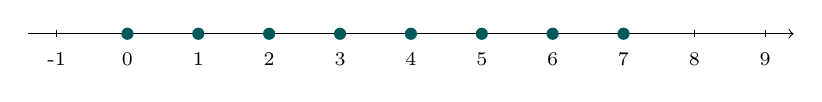
\begin{tikzpicture}[x=0.9cm,y=0.55cm]
    \draw[->] (-1.4,0) -- (9.4,0);
    \foreach \x in {-1,...,9} {\draw (\x,0.08)--(\x,-0.08) node[below=2pt]{\scriptsize\x};}
    \foreach \x in {0,...,7} {\fill[teal!70!black] (\x,0) circle (2.2pt);}
  \end{tikzpicture}
  \caption{3 位无符号整数格式的可表示数在数轴上的位置。依据原书图 A.3 重绘。}
  \label{fig:a-3}
\end{figure}

浮点格式的可表示数也可以用类似方式观察。图 \ref{fig:a-4} 给出目前讨论的格式及其两个
变体的全部可表示数。为了控制表格大小，这里采用 5 位格式：1 位 $S$、2 位 $E$（移 1 码）
和 2 位 $M$（省略 ``$1.$'' 部分）。“无零”列给出前文格式的可表示数。建议读者使用第
\ref{sec:appa-floating-point-representation} 节的公式，至少自行生成“无零”列的一部分。
注意，这种格式不能表示 0。

\begin{figure}[htbp]
  \centering
  \scriptsize
  \setlength{\tabcolsep}{2.2pt}
  \resizebox{\linewidth}{!}{%
  \begin{tabular}{cc|cc|cc|cc}
    \hline
    $E$ & $M$ & \multicolumn{2}{c|}{\textbf{无零}} &
      \multicolumn{2}{c|}{\textbf{突发下溢}} & \multicolumn{2}{c}{\textbf{反规格化}}\\
    &&$S=0$&$S=1$&$S=0$&$S=1$&$S=0$&$S=1$\\
    \hline
    00&00&$2^{-1}$&$-(2^{-1})$&0&0&0&0\\
    00&01&$2^{-1}+1\cdot2^{-3}$&$-(2^{-1}+1\cdot2^{-3})$&0&0&$1\cdot2^{-2}$&$-1\cdot2^{-2}$\\
    00&10&$2^{-1}+2\cdot2^{-3}$&$-(2^{-1}+2\cdot2^{-3})$&0&0&$2\cdot2^{-2}$&$-2\cdot2^{-2}$\\
    00&11&$2^{-1}+3\cdot2^{-3}$&$-(2^{-1}+3\cdot2^{-3})$&0&0&$3\cdot2^{-2}$&$-3\cdot2^{-2}$\\
    \hline
    01&00&$2^0$&$-(2^0)$&$2^0$&$-(2^0)$&$2^0$&$-(2^0)$\\
    01&01&$2^0+1\cdot2^{-2}$&$-(2^0+1\cdot2^{-2})$&$2^0+1\cdot2^{-2}$&$-(2^0+1\cdot2^{-2})$&$2^0+1\cdot2^{-2}$&$-(2^0+1\cdot2^{-2})$\\
    01&10&$2^0+2\cdot2^{-2}$&$-(2^0+2\cdot2^{-2})$&$2^0+2\cdot2^{-2}$&$-(2^0+2\cdot2^{-2})$&$2^0+2\cdot2^{-2}$&$-(2^0+2\cdot2^{-2})$\\
    01&11&$2^0+3\cdot2^{-2}$&$-(2^0+3\cdot2^{-2})$&$2^0+3\cdot2^{-2}$&$-(2^0+3\cdot2^{-2})$&$2^0+3\cdot2^{-2}$&$-(2^0+3\cdot2^{-2})$\\
    \hline
    10&00&$2^1$&$-(2^1)$&$2^1$&$-(2^1)$&$2^1$&$-(2^1)$\\
    10&01&$2^1+1\cdot2^{-1}$&$-(2^1+1\cdot2^{-1})$&$2^1+1\cdot2^{-1}$&$-(2^1+1\cdot2^{-1})$&$2^1+1\cdot2^{-1}$&$-(2^1+1\cdot2^{-1})$\\
    10&10&$2^1+2\cdot2^{-1}$&$-(2^1+2\cdot2^{-1})$&$2^1+2\cdot2^{-1}$&$-(2^1+2\cdot2^{-1})$&$2^1+2\cdot2^{-1}$&$-(2^1+2\cdot2^{-1})$\\
    10&11&$2^1+3\cdot2^{-1}$&$-(2^1+3\cdot2^{-1})$&$2^1+3\cdot2^{-1}$&$-(2^1+3\cdot2^{-1})$&$2^1+3\cdot2^{-1}$&$-(2^1+3\cdot2^{-1})$\\
    \hline
    11&\multicolumn{7}{c}{保留模式}\\
    \hline
  \end{tabular}}
  \caption{无零、突发下溢和反规格化格式的可表示数。依据原书图 A.4 重绘。}
  \label{fig:a-4}
\end{figure}

从图 \ref{fig:a-5} 所示的数轴上观察这些可表示数，还能获得更多认识。图中只画出正的
可表示数；负数关于 0 与相应的正数对称。

\begin{figure}[htbp]
  \centering
  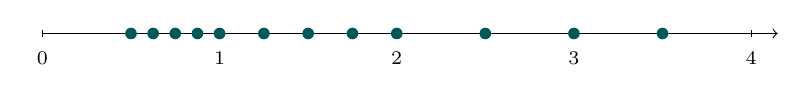
\begin{tikzpicture}[x=2.25cm,y=0.55cm]
    \draw[->] (0,0)--(4.15,0);
    \foreach \x in {0,1,2,3,4}{\draw (\x,0.08)--(\x,-0.08) node[below=2pt]{\scriptsize\x};}
    \foreach \x in {0.5,0.625,0.75,0.875,1,1.25,1.5,1.75,2,2.5,3,3.5}
      {\fill[teal!70!black] (\x,0) circle (2.1pt);}
  \end{tikzpicture}
  \caption{无零表示中的正可表示数。依据原书图 A.5 重绘。}
  \label{fig:a-5}
\end{figure}

可以得到五点观察。第一，指数位定义可表示数的主要区间。图 \ref{fig:a-5} 的指数有 2 位，
因此 0 的每一侧都有三个主要区间。主要区间基本都位于相邻的 2 的幂之间。2 位指数中有一个
保留位模式 11，所以存在三个 2 的幂：$2^{-1}=0.5_D$、$2^0=1.0_D$ 和 $2^1=2.0_D$，
每个幂都是一个可表示数区间的起点。0 左侧还有三个未在图中画出的 2 的幂：
$-2^{-1}=-0.5_D$、$-2^0=-1.0_D$ 和 $-2^1=-2.0_D$。

第二，尾数位定义每个区间内可表示数的数量。2 位尾数使每个区间包含 4 个可表示数。一般
而言，$N$ 位尾数使每个区间包含 $2^N$ 个可表示数。待表示的数若落在两个可表示数之间，就
会舍入到其中一个。显然，每个区间内的可表示数越多，就越能精确表示该区域中的数。因此，
尾数位数决定表示的精度。

第三，这种格式不能表示 0。图 \ref{fig:a-4} 的“无零”列和图 \ref{fig:a-5} 的可表示数中
都缺少 0。0 是最重要的数之一，无法表示 0 是一种数值表示系统的严重缺陷，稍后将处理它。

第四，越接近 0，可表示数之间的距离越小。向 0 移动时，每个区间的宽度都是前一个区间的
一半。图 \ref{fig:a-5} 最右侧区间宽 2，下一个区间宽 1，再下一个宽 0.5。图中未画出的
0 左侧也有三个包含负可表示数的区间：最左侧宽 2，下一个宽 1，再下一个宽 0.5。由于每个
区间包含相同数量的可表示数，即图中的 4 个，所以越接近 0，可表示数越密集。换言之，数的
绝对值越小，相邻可表示数就越接近。这是一种理想趋势，因为绝对值越小，精确表示往往越
重要。相邻可表示数之间的距离决定落在该区间内的数可能产生的最大舍入误差。例如，如果银行
账户有十亿美元，计算余额时一美元的舍入误差甚至可能不易察觉；但余额总共只有十美元时，
一美元的舍入误差就十分明显。

第五，遗憾的是，越靠近 0、可表示数越密集、表示精度越高的趋势并没有延续到 0 的紧邻区域。
0 附近存在一个可表示数空隙，这是规格化尾数的范围排除 0 所致，也是另一项严重缺陷。表示
0 到 0.5 之间的数时，这种格式产生的误差明显比表示 0.5 到 1.0 之间较大数值时高 4 倍。
一般而言，若尾数有 $m$ 位，这种表示方式在最接近 0 的区间内产生的误差会是相邻区间的
$2^m$ 倍。某些数值方法依靠很小的数据值准确检测收敛条件，这种缺陷会使执行时间和结果
准确度不稳定。此外，有些算法会产生很小的数，并最终把它们用作分母；表示这些小数时产生的
误差可能在除法中被大幅放大，导致算法数值不稳定。

把 0 纳入规格化浮点数系统的一种方法是\textbf{突发下溢（abrupt underflow）}约定，见图
\ref{fig:a-4} 第二组数据列。只要 $E=0$，就把数解释为 0。在 5 位格式中，这种方法移除了
0 附近（$-1.0$ 到 $+1.0$ 之间）的 8 个可表示数，即 4 个正数和 4 个负数，并把它们全部
变为 0。由于实现简单，20 世纪 80 年代的一些小型机采用了突发下溢。直至今天，某些要求高速
运行的算术单元仍使用这一约定。它虽然使 0 成为可表示数，却在 0 附近形成更大的可表示数
空隙，如图 \ref{fig:a-6} 所示。与图 \ref{fig:a-5} 相比，0.5 到 1.0 之间的空隙显著扩大
了 2 倍。正如前文所述，许多数值算法的正确性依赖对接近 0 的小数进行准确表示，这一空隙
会给它们造成问题。

\begin{figure}[htbp]
  \centering
  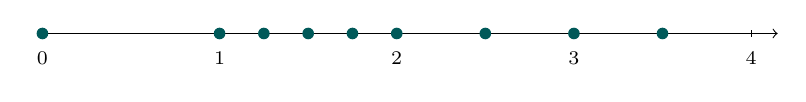
\begin{tikzpicture}[x=2.25cm,y=0.55cm]
    \draw[->] (0,0)--(4.15,0);
    \foreach \x in {0,1,2,3,4}{\draw (\x,0.08)--(\x,-0.08) node[below=2pt]{\scriptsize\x};}
    \foreach \x in {0,1,1.25,1.5,1.75,2,2.5,3,3.5}{\fill[teal!70!black] (\x,0) circle (2.1pt);}
  \end{tikzpicture}
  \caption{突发下溢格式的正可表示数。依据原书图 A.6 重绘。}
  \label{fig:a-6}
\end{figure}

IEEE 标准实际采用的方法称为\textbf{反规格化（denormalization）}。它放宽了非常接近 0
的数必须规格化的要求。如图 \ref{fig:a-4} 所示，只要 $E=0$，尾数就不再假定为 $1.XX$
形式，而是假定为 $0.XX$；指数值则假定与前一个区间相同。例如，图 \ref{fig:a-4} 中的
反规格化表示 00001 具有指数值 00 和尾数值 01。尾数解释为 0.01，指数值解释为与前一个
区间相同的 0，而不是 $-1$。因此，00001 现在表示
$0.01\times2^0=2^{-2}$。图 \ref{fig:a-7} 给出反规格化格式的可表示数。现在，0 的紧邻
区域内均匀分布着可表示数。直观地说，反规格化约定把无零表示最后一个区间中的 4 个数摊开，
用它们覆盖原有空隙，从而消除了前两种方法中的不理想空隙。最后两个区间内，相邻可表示数的
距离实际上完全相同。一般而言，若 $n$ 位指数为 0，则数值为
\[
  0.M\cdot2^{-2^{n-1}+2}.
\]

\noindent\textbf{译者注：}底本上述段落写作“如图 A.6 所示，只要 $E=0$”，但图 A.6
只是突发下溢格式的数轴；展示 $E=0$ 三种解释的是图 A.4。本译稿按实际图意修正引用。

\begin{figure}[htbp]
  \centering
  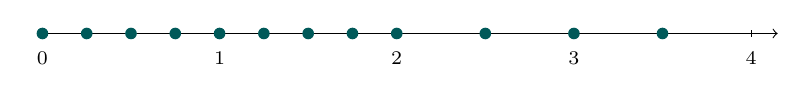
\begin{tikzpicture}[x=2.25cm,y=0.55cm]
    \draw[->] (0,0)--(4.15,0);
    \foreach \x in {0,1,2,3,4}{\draw (\x,0.08)--(\x,-0.08) node[below=2pt]{\scriptsize\x};}
    \foreach \x in {0,0.25,0.5,0.75,1,1.25,1.5,1.75,2,2.5,3,3.5}
      {\fill[teal!70!black] (\x,0) circle (2.1pt);}
  \end{tikzpicture}
  \caption{反规格化格式的正可表示数。依据原书图 A.7 重绘。}
  \label{fig:a-7}
\end{figure}

反规格化公式相当复杂。硬件还必须检测一个数是否落在反规格化区间，并为它选择合适的表示。
高速实现反规格化可能需要大量硬件；硬件规模适中的实现每次生成或使用反规格化数时，常会
引入数千个时钟周期的延迟。这正是早期 CUDA 设备不支持反规格化的原因。不过，较新制程
提供了更多可用晶体管，近代各代 CUDA 设备几乎都已支持反规格化\cite{appa-cuda-fp}。
CUDA 程序员可以设置 NVCC 编译器标志 \code{ftz=true}（开启）或 \code{ftz=false}
（关闭），控制 GPU 算术单元是否使用反规格化。

总之，浮点表示的精度由把浮点数表示为某个可表示数时可能引入的最大误差衡量。误差越小，
精度越高。增加尾数位可以提高浮点表示精度；尾数每增加一位，最大误差减半。因此，使用更多
尾数位的数值系统具有更高精度，IEEE 标准中的双精度数与单精度数正体现了这一点。

\section{IEEE 格式的精度和特殊位模式}
\label{sec:appa-ieee-precision}

下面进一步考察实际 IEEE 格式的细节。IEEE 格式主要有两个精度级别。单精度（single
precision，sp）数共 32 位，包括 1 位 $S$、8 位 $E$ 和 23 位 $M$；双精度（double
precision，dp）数共 64 位，包括 1 位 $S$、11 位 $E$ 和 52 位 $M$。双精度数的尾数多
29 位，所以表示一个数时的最大舍入误差降为单精度格式的 $1/2^{29}$。指数多出的 3 位还把
指数编码所能划分的区间数扩大为 $2^3=8$ 倍。由此，可表示数的范围同时向极大值和极小值
延伸。例如，宇宙中的原子总数估计为 $10^{80}$，而双精度格式最大可以表示 $10^{308}$。

\noindent\textbf{译者注：}底本写作“区间数增加 $2^{2^3}=256$ 倍”。8 位指数增加到
11 位时，指数位模式数量增加 $2^3=8$ 倍，而不是 256 倍；本译稿按位模式数量作最小修正。

\begin{figure}[htbp]
  \centering
  \small
  \begin{tabular}{ccc}
    \hline
    \textbf{指数} & \textbf{尾数} & \textbf{含义}\\
    \hline
    $11\ldots1$ & $\ne0$ & NaN\\
    $11\ldots1$ & $=0$ & $(-1)^S\times\infty$\\
    $00\ldots0$ & $\ne0$ & 反规格化数\\
    $00\ldots0$ & $=0$ & 0\\
    \hline
  \end{tabular}
  \caption{IEEE 标准格式中的特殊位模式。依据原书图 A.8 重绘。}
  \label{fig:a-8}
\end{figure}

IEEE 浮点格式的特殊位模式见图 \ref{fig:a-8}。当指数位全为 1 且尾数为 0 时，所表示的数
为无穷。所有可表示数都位于 $-\infty$（负无穷）与 $+\infty$（正无穷）之间。溢出可以产生
$\infty$，例如用一个大数除以一个很小的数。也就是说，浮点算术操作产生超出可表示数范围的
数值时，输出会饱和到正无穷或负无穷；这与整数算术不同，后者的结果超出可表示范围时会发生
回绕或产生未定义值。任何可表示数除以 $+\infty$ 或 $-\infty$ 都得到 0。

当指数位全为 1 而尾数不为 0 时，所表示的是\textbf{非数（Not a Number，NaN）}。输入值
在数学上未定义的操作会产生 NaN，例如 $0/0$、$0\times\infty$、$\infty/\infty$ 和
$\infty-\infty$；NaN 也用于表示程序中没有正确初始化的数据。IEEE 标准定义了两类 NaN：
信令 NaN 和静默 NaN。信令 NaN（signaling NaN，SNaN）的最高尾数位应当清零，静默 NaN
（quiet NaN，QNaN）的最高尾数位则置位。

信令 NaN 用作算术操作输入时会触发异常。例如，$(1.0+\text{signaling NaN})$ 会向操作系统
发出异常信号。程序员希望一旦浮点计算使用任何 NaN，程序执行就被中断时，会采用信令 NaN。
这种情况通常意味着程序执行出了问题。在任务关键型应用中，必须通过独立手段验证执行有效性，
之后才能继续。例如，软件工程师常把所有未初始化数据表示成信令 NaN，以保证程序执行期间能
检测到未初始化数据的使用。当前一代 GPU 硬件不支持信令 NaN，原因是在大规模并行执行中
很难准确发出异常信号。

静默 NaN 用作算术操作输入时不会触发异常，而是产生另一个静默 NaN。例如，
$(1.0+\text{quiet NaN})$ 会产生静默 NaN。静默 NaN 常用于允许用户检查输出，并判断是否
应换一组输入重新运行应用、以获得更有效结果的场景。打印结果时，静默 NaN 会显示为
``NaN''，用户可以在输出文件中轻易发现它们。

NaN 可能对应许多位模式。例如，在单精度格式中，最高尾数位用于区分信令与静默，所以有
$2^{22}-1$ 种可能的 NaN 尾数位模式。其中一些模式可以进一步用来说明产生 NaN 的原因。

\section{算术准确度与舍入}
\label{sec:appa-accuracy-rounding}

理解 IEEE 浮点格式以后，可以讨论算术准确度。精度由浮点数格式使用的尾数位数决定，准确度
则由对浮点数执行的操作决定。浮点算术操作的准确度由该操作引入的最大误差衡量；误差越小，
准确度越高。浮点算术最常见的误差来源，是操作产生无法精确表示的结果，因而必须舍入。结果
尾数需要的位数超过格式所能容纳的位数时，就会发生舍入。例如，乘法得到的乘积位数是任一
输入值位数的两倍。又如，两个指数相同的浮点值相加时，可以直接把尾数相加；若两个输入操作
数的指数不同，就必须反复把指数较小者的尾数除以 2（即全部尾数位右移一位），并把其指数
加 1，直至两个指数相等。因此，最终结果可能拥有格式无法容纳的更多位。

可以用图 \ref{fig:a-4} 的 5 位表示说明操作数的对齐移位。假设要把
$1.00_B\times2^{-2}$（0, 00, 01）加到 $1.00_B\times2^1$（0, 10, 00）上，即计算
$1.00_B\times2^1+1.00_B\times2^{-2}$。由于指数不同，第二个数的尾数必须右移 3 位，
相加式变为
$1.00_B\times2^1+0.001_B\times2^1$。现在可以把尾数相加，理想结果是
$1.001_B\times2^1$。然而，它不是 5 位表示中的可表示数：理想结果需要 3 位尾数，而格式
只有 2 位。因此，最多只能产生两个最接近的可表示数之一，即 $1.01_B\times2^1$ 或
$1.00_B\times2^1$。这样会引入 $0.001_B\times2^1$ 的误差，等于最低有效位位值的一半，
称为 $0.5_D$ ULP（Units in the Last Place，末位单位）。也可以把 ULP 看作给定格式中
两个相邻可表示数之间的间隔。若硬件能完美地执行算术和舍入，引入的误差就不应超过
$0.5_D$ ULP。据我们所知，目前所有 CUDA 设备都能达到这一准确度。

实际中，除法和超越函数等较复杂的硬件算术单元通常采用多项式近似算法。若近似采用的项数
不足，结果误差可能超过 $0.5_D$ ULP。例如，求倒数操作的理想结果为
$1.00_B\times2^1$，但硬件因使用近似算法而产生 $1.10_B\times2^1$，则误差为 2 ULP，
因为误差 $1.10_B-1.00_B=0.10_B$ 是末位单位 $0.01_B$ 的两倍。实际中，一些早期设备的
硬件求倒数操作会引入尾数最低位位值两倍的误差，即 2 ULP。较新一代 CUDA 设备拥有更多
晶体管，其硬件算术操作在数学上准确，并遵循 IEEE 标准\cite{appa-cuda-fp}。

\section{较低精度格式}
\label{sec:appa-lower-precision}

有些应用天然使用较小的输入数据类型，如 4 位、6 位、8 位和 16 位类型。医学成像、遥感、
射电天文学、地震分析和其他处理自然数据的应用经常属于此类。近年来，LLM 等深度学习模型
也开始使用较小的浮点数据类型。这些应用的数据表示只需要少量有效位，却能从浮点格式较大的
可表示数范围中获益，因而推动了小于单精度的浮点格式。较小格式能减少每次算术操作读取的
字节数，从而提高这些应用的计算强度。

近代 GPU 架构引入了对 16 位、8 位和 4 位浮点计算的硬件支持，以提高能够容忍低精度算术
的应用的性能和能源效率\cite{appa-ocp-mx}。例如，H100 使用 Tensor Core 执行 8 位浮点
（FP8）算术时吞吐量为 3,958 TFLOPS，相比使用 Tensor Core 的单精度吞吐量
989 TFLOPS 有显著提升。

\section{算法方面的考量}
\label{sec:appa-algorithm-considerations}

数值算法经常需要对大量数值求和。例如，矩阵乘法的点积需要对输入矩阵元素的成对乘积求和。
理想情况下，加法满足结合律，求和次序不应影响最终总和；但在有限精度下，求和次序会影响
最终结果的准确度。假设需要在 5 位表示中对四个数执行求和归约：
\[
  1.00_B\times2^0+1.00_B\times2^0+1.00_B\times2^{-2}+1.00_B\times2^{-2}.
\]
如果严格按照顺序相加，操作序列为
\begin{align*}
  &1.00_B\times2^0+1.00_B\times2^0+1.00_B\times2^{-2}+1.00_B\times2^{-2}\\
  &\quad=1.00_B\times2^1+1.00_B\times2^{-2}+1.00_B\times2^{-2}\\
  &\quad=1.00_B\times2^1+1.00_B\times2^{-2}
   =1.00_B\times2^1.
\end{align*}
第二步和第三步中，较小的操作数与较大操作数相比过小，因而直接消失。

再考虑一种并行算法：并行地把前两个值相加、把后两个操作数相加，然后再求两组部分和之和：
\begin{align*}
  &(1.00_B\times2^0+1.00_B\times2^0)
    +(1.00_B\times2^{-2}+1.00_B\times2^{-2})\\
  &\quad=1.00_B\times2^1+1.00_B\times2^{-1}
   =1.01_B\times2^1.
\end{align*}
读者应能看出，这种算法实现了第 10 章介绍的归约树，并假定加法满足结合律。它与顺序算法
得到的结果不同，因为第三个值与第四个值的和已经足够大，能够影响后续加法。不了解浮点精度
和准确度问题的应用开发者，常会对顺序算法与并行算法之间的这种差异感到意外。

上述情形中，并行算法产生的结果比顺序算法更准确；读者也应能稍作改变，构造出并行算法不如
顺序算法准确的情形。换言之，对浮点数而言，加法并不严格满足结合律。经验丰富的应用开发者
要么确保最终结果的变化处于可容忍范围，要么以适当方式对数据排序或分组，使并行算法得到
尽可能准确的结果。

在归约计算前预先排序数据，是尽量提高浮点算术准确度的常见技术。在求和归约示例中，若按
数值升序预先排序数据，将得到
\[
  1.00_B\times2^{-2}+1.00_B\times2^{-2}+1.00_B\times2^0+1.00_B\times2^0.
\]
并行算法把数值分组时，例如把前两个数分为一组、后两个数分为另一组，同一组中数值的大小
就彼此接近。显然，预排序时还必须考虑数值的符号。这样，在各组内执行加法时，结果通常会
更准确。此外，一些并行算法让每个线程在组内顺序归约数值；按升序排列数值也能提高这种顺序
加法的准确度。这正是大规模并行数值算法经常使用排序的一个原因。有兴趣的读者可以进一步
研究补偿求和算法，也称 Kahan 求和算法，它能以更稳健的方式准确求和浮点值
\cite{appa-kahan}。

\section{线性求解器与数值稳定性}
\label{sec:appa-linear-solvers}

操作次序会改变归约的数值结果，对线性方程组求解器等某些计算而言，后果可能更加严重。在
这些求解器中，不同的输入数值可能需要采用不同操作次序才能找到解。算法若没有针对某组输入
遵循所需的操作次序，即使解存在，也可能无法求出。只要任意给定输入存在解，就总能找到合适
操作次序并求出解的算法称为\textbf{数值稳定（numerically stable）}算法；做不到这一点的
算法称为\textbf{数值不稳定（numerically unstable）}算法。

数值稳定性有时会增加为计算问题寻找高效并行算法的难度。下面用基于高斯消元的求解器说明：
\[
\begin{aligned}
  3X+5Y+2Z&=19 &&\text{（方程 1）},\\
  2X+3Y+Z&=11 &&\text{（方程 2）},\\
  X+2Y+2Z&=11 &&\text{（方程 3）}.
\end{aligned}
\]
只要这三个方程表示的平面存在交点，就可以用高斯消元求得交点坐标。图 \ref{fig:a-9} 展示
了过程，其中各变量从位置较低的方程中依次消去。

\begin{figure}[htbp]
  \centering
  \scriptsize
  \renewcommand{\arraystretch}{1.15}
  \begin{tabular}{c@{\ $\Longrightarrow$\ }c}
    $\begin{aligned}3X+5Y+2Z&=19\\2X+3Y+Z&=11\\X+2Y+2Z&=11\end{aligned}$
      & $\begin{aligned}X+\frac53Y+\frac23Z&=\frac{19}3\\X+\frac32Y+\frac12Z&=\frac{11}2\\X+2Y+2Z&=11\end{aligned}$\\
    原方程 & 步骤 1：各方程除以 $X$ 的系数\\[0.7em]
    $\begin{aligned}X+\frac53Y+\frac23Z&=\frac{19}3\\-\frac16Y-\frac16Z&=-\frac56\\\frac13Y+\frac43Z&=\frac{14}3\end{aligned}$
      & $\begin{aligned}X+\frac53Y+\frac23Z&=\frac{19}3\\Y+Z&=5\\Y+4Z&=14\end{aligned}$\\
    步骤 2：从方程 2、3 减去方程 1 & 步骤 3：方程 2 除以 $-1/6$，方程 3 除以 $1/3$\\[0.7em]
    $\begin{aligned}X+\frac53Y+\frac23Z&=\frac{19}3\\Y+Z&=5\\3Z&=9\end{aligned}$
      & $\begin{aligned}X+\frac53Y+\frac23Z&=\frac{19}3\\Y+Z&=5\\Z&=3\end{aligned}$\\
    步骤 4：方程 3 减去方程 2 & 步骤 5：方程 3 除以 3，求得 $Z$\\[0.7em]
    $\begin{aligned}X+\frac53Y+\frac23Z&=\frac{19}3\\Y&=2\\Z&=3\end{aligned}$
      & $\begin{aligned}X&=1\\Y&=2\\Z&=3\end{aligned}$\\
    步骤 6：把 $Z$ 回代方程 2，求得 $Y$ & 步骤 7：把 $Y,Z$ 回代方程 1，求得 $X$
  \end{tabular}
  \caption{用高斯消元和回代求解线性方程组。依据原书图 A.9 重绘。}
  \label{fig:a-9}
\end{figure}

第一步中，所有方程分别除以各自的 $X$ 系数：方程 1 除以 3，方程 2 除以 2，方程 3 除以
1，使所有方程的 $X$ 系数相同。第二步从方程 2 和方程 3 中减去方程 1，从而消去二者中的
$X$，如图 \ref{fig:a-9} 所示。

现在可以把方程 2 和方程 3 看作变量比原方程组少一个的小型方程组。由于它们不含 $X$，可以
独立于方程 1 求解。第三步再消去方程 3 中的 $Y$：方程 2 除以其 $Y$ 系数 $-1/6$，方程 3
除以其 $Y$ 系数 $1/3$，使两个方程的 $Y$ 系数相同。第四步从方程 3 中减去方程 2，消去
方程 3 中的 $Y$。

含有更多方程的系统需要继续重复这一过程。本例只有三个变量，第三个方程最终只含 $Z$；把
方程 3 除以 $Z$ 的系数即可得到 $Z=3$。把 $Z$ 回代方程 2，得到 $Y=2$；再把 $Z=3$ 和
$Y=2$ 回代方程 1，得到 $X=1$，至此得到原方程组的完整解。步骤 6 和步骤 7 构成方法的
第二阶段，称为\textbf{回代（backward substitution）}：从最后一个方程反向回到第一个
方程，逐步求出更多变量。

实际中，计算机会以矩阵形式存储方程。全部计算只涉及系数和等号右侧的值，所以只需把这些值
存入矩阵。图 \ref{fig:a-10} 从矩阵视角展示高斯消元和回代过程。矩阵的每一行对应一个原始
方程，对方程的操作变为对矩阵行的操作。

\begin{figure}[htbp]
  \centering
  \scriptsize
  \renewcommand{\arraystretch}{1.15}
  \begin{tabular}{c@{\ $\Longrightarrow$\ }c}
    $\left[\begin{array}{ccc|c}3&5&2&19\\2&3&1&11\\1&2&2&11\end{array}\right]$
      & $\left[\begin{array}{ccc|c}1&5/3&2/3&19/3\\1&3/2&1/2&11/2\\1&2&2&11\end{array}\right]$\\
    原矩阵 & 步骤 1\\[0.5em]
    $\left[\begin{array}{ccc|c}1&5/3&2/3&19/3\\0&-1/6&-1/6&-5/6\\0&1/3&4/3&14/3\end{array}\right]$
      & $\left[\begin{array}{ccc|c}1&5/3&2/3&19/3\\0&1&1&5\\0&1&4&14\end{array}\right]$\\
    步骤 2 & 步骤 3\\[0.5em]
    $\left[\begin{array}{ccc|c}1&5/3&2/3&19/3\\0&1&1&5\\0&0&3&9\end{array}\right]$
      & $\left[\begin{array}{ccc|c}1&5/3&2/3&19/3\\0&1&1&5\\0&0&1&3\end{array}\right]$\\
    步骤 4 & 步骤 5\\[0.5em]
    $\left[\begin{array}{ccc|c}1&5/3&2/3&19/3\\0&1&0&2\\0&0&1&3\end{array}\right]$
      & $\left[\begin{array}{ccc|c}1&0&0&1\\0&1&0&2\\0&0&1&3\end{array}\right]$\\
    步骤 6 & 步骤 7
  \end{tabular}
  \caption{矩阵视角下的高斯消元和回代。依据原书图 A.10 重绘。}
  \label{fig:a-10}
\end{figure}

高斯消元后，矩阵变成三角矩阵。由于物理和数学方面的多种原因，这是一类非常常见的矩阵。
最终目标是把矩阵的系数部分变为对角形式，每行在对角线上只有一个值 1。这称为单位矩阵，
因为任意矩阵与单位矩阵相乘仍为自身。这也说明了为什么对一个矩阵执行高斯消元，等价于用
该矩阵的逆矩阵乘它。

为图 \ref{fig:a-10} 所述高斯消元过程设计并行算法并不困难。例如，可以编写 CUDA 内核，
指定每个线程完成矩阵某一行上的全部计算。若方程组系数能装入共享内存，可以用一个线程块
执行高斯消元。所有线程共同迭代各步骤；每次除法后，所有线程参与屏障同步，然后共同执行
减法。一次减法之后，一个线程会停止参与，因为它负责的行在回代阶段以前不再有工作。减法
之后，所有线程还要再次执行屏障同步，保证下一步采用更新后的信息。方程组包含很多变量时，
这种并行执行有望取得可观加速。

遗憾的是，前述简单高斯消元算法可能数值不稳定。考虑下面的例子：
\[
\begin{aligned}
  5Y+2Z&=16 &&\text{（方程 1）},\\
  2X+3Y+Z&=11 &&\text{（方程 2）},\\
  X+2Y+2Z&=11 &&\text{（方程 3）}.
\end{aligned}
\]
执行算法的第一步时就会遇到问题：方程 1 中 $X$ 的系数为 0，不能用 $X$ 的系数除方程 1，
也无法通过从方程 2 和方程 3 中减去方程 1 来消去二者的 $X$。读者可以验证，这个方程组
存在解，而且仍为 $X=1,Y=2,Z=3$。因此，该算法数值不稳定：某些输入值下即使解存在，
它也可能无法产生解。

更隐蔽的问题出现在某一步主变量的系数很小，而且它可能已经受到上一次迭代舍入误差影响时。
用这个很小且不准确的值去除其余系数，可能给后续步骤乃至最终解引入更大的误差。因此，算法
的数值不稳定性常以误差在各步骤中的增长程度衡量。

这是高斯消元算法的一个著名问题，可以用通常所称的\textbf{选主元（pivoting）}方法解决。
其思想是在剩余方程中找出一个主变量系数不为 0、而且绝对值最好较大的方程；把当前最上方
的方程与所选方程交换以后，算法便能成功且更准确地从其余方程中消去主变量。对上述三个方程
选主元后得到
\[
\begin{aligned}
  2X+3Y+Z&=11 &&\text{（方程 $1'$，原方程 2）},\\
  5Y+2Z&=16 &&\text{（方程 $2'$，原方程 1）},\\
  X+2Y+2Z&=11 &&\text{（方程 $3'$，原方程 3）}.
\end{aligned}
\]
方程 $1'$ 中 $X$ 的系数不再为 0，可以继续执行高斯消元，如图 \ref{fig:a-11} 所示。

\begin{figure}[htbp]
  \centering
  \scriptsize
  \renewcommand{\arraystretch}{1.15}
  \begin{tabular}{c@{\ $\Longrightarrow$\ }c}
    $\left[\begin{array}{ccc|c}0&5&2&16\\2&3&1&11\\1&2&2&11\end{array}\right]$
      & $\left[\begin{array}{ccc|c}2&3&1&11\\0&5&2&16\\1&2&2&11\end{array}\right]$\\
    原矩阵 & 选主元：交换第 1、2 行\\[0.5em]
    $\left[\begin{array}{ccc|c}1&3/2&1/2&11/2\\0&5&2&16\\1&2&2&11\end{array}\right]$
      & $\left[\begin{array}{ccc|c}1&3/2&1/2&11/2\\0&5&2&16\\0&1/2&3/2&11/2\end{array}\right]$\\
    步骤 1：第 1 行除以 2 & 步骤 2：第 3 行减去第 1 行\\[0.5em]
    $\left[\begin{array}{ccc|c}1&3/2&1/2&11/2\\0&1&2/5&16/5\\0&1&3&11\end{array}\right]$
      & $\left[\begin{array}{ccc|c}1&3/2&1/2&11/2\\0&1&2/5&16/5\\0&0&13/5&39/5\end{array}\right]$\\
    步骤 3 & 步骤 4\\[0.5em]
    $\left[\begin{array}{ccc|c}1&3/2&1/2&11/2\\0&1&2/5&16/5\\0&0&1&3\end{array}\right]$
      & $\left[\begin{array}{ccc|c}1&3/2&1/2&11/2\\0&1&0&2\\0&0&1&3\end{array}\right]$\\
    步骤 5：求得 $Z$ & 步骤 6：求得 $Y$\\[0.5em]
    \multicolumn{2}{c}{$\left[\begin{array}{ccc|c}1&0&0&1\\0&1&0&2\\0&0&1&3\end{array}\right]$}\\
    \multicolumn{2}{c}{步骤 7：求得 $X$}
  \end{tabular}
  \caption{带选主元的高斯消元。依据原书图 A.11 重绘。}
  \label{fig:a-11}
\end{figure}

\noindent\textbf{译者注：}底本图 A.11 的第 5 步把第一行写成
$[1,5/3,2/3\mid19/3]$，这是图 A.10 中前一个方程组的数据；对本例而言，该行应继续保持为
$[1,3/2,1/2\mid11/2]$。本译稿按步骤 1 的结果重绘，后续回代结果不变。

读者应逐步检查图 \ref{fig:a-11}。这里最重要的新认识是，有些方程可能不含算法当前正在
消去的变量（例如图中步骤 1 的第 2 行），负责该方程的线程便不需要执行除法。

一般而言，选主元步骤应在所有主变量中选择系数绝对值最大的方程，把该方程（行）与当前最上
方的方程交换，并把相应变量（列）与当前变量交换。选主元在概念上很简单，却可能显著增加
实现复杂度和性能开销。回忆简单 CUDA 内核中每个线程分配一行；选主元需要检查、并且可能
交换分散在这些线程之间的系数数据。若所有系数都位于共享内存中，这并非大问题：只要控制
warp 内的控制流分歧程度，就可以由块内线程执行并行最大值归约。

然而，若一个线性方程组由多个线程块、甚至计算集群的多个节点共同求解，检查分散在多个线程
块或多个集群节点上的数据就可能极其昂贵。这正是\textbf{通信规避算法（communication-
avoiding algorithm）}避免选主元式全局数据检查的主要动机\cite{appa-ballard}。这一问题
通常有两种处理方法。部分选主元把交换候选项限制在局部方程集合中，以控制全局检查成本，
代价是可能略微降低解的数值准确度。研究人员还证明，随机化往往也能让解保持很高的数值
准确度。

\section{小结}
\label{sec:appa-summary}

本附录介绍了理解精度所需的基础概念，包括浮点格式和可表示数；并以此为基础说明反规格化数，
以及它们为何对许多数值应用十分重要。早期 CUDA 设备不支持反规格化数，后续硬件世代则已
提供支持。我们还解释了浮点操作的算术准确度。CUDA 程序员必须理解这一点，才能认识特殊
函数单元实现的快速算术操作可能具有较低准确度。更重要的是，读者现在应当理解并行算法为何
经常影响计算结果的准确度，以及如何利用排序和其他技术提高计算准确度。

\section{练习}
\label{sec:appa-exercises}

\begin{enumerate}[label=\arabic*.,leftmargin=2.7em]
  \item 为一种 6 位格式（1 位符号、3 位尾数、2 位指数）绘制与图 \ref{fig:a-5} 等价的
  图。用结果说明尾数每增加一位，会如何改变数轴上的可表示数集合。

  \item 为另一种 6 位格式（1 位符号、2 位尾数、3 位指数）绘制与图 \ref{fig:a-5} 等价
  的图。用结果说明指数每增加一位，会如何改变数轴上的可表示数集合。

  \item 假设一种新处理器受技术困难限制，执行加法的浮点算术单元只能“向零舍入”（通过向
  0 截断数值来舍入）。硬件保留了足够多的位，唯一误差来自舍入。这台机器上加法操作的最大
  ULP 误差是多少？

  \item 一名研究生编写了 CUDA 内核，把一个大型浮点数组归约为所有元素之和。数组总是按
  数值从小到大排序。为避免分支分歧，他决定实现图 \ref{fig:10-7} 的算法。请解释这为何
  会降低结果的准确度。

  \par\noindent\textbf{译者注：}底本本题写作“图 A.4 的算法”，但图 A.4 是浮点可表示
  数表，并非归约算法。按“避免分支分歧”和第 10 章的上下文，本题实际指向图 10.7 所示、
  由图 10.8 内核实现的低分歧归约分配方式；本译稿据此修正。

  \item 假设某算术单元以迭代近似算法实现 \code{sin()} 函数，每个时钟周期为结果再产生
  2 个准确的尾数位。架构师决定让该算术函数迭代 9 个时钟周期。假设硬件把剩余尾数位全部
  填为 0。对于 IEEE 单精度数，这一 \code{sin()} 硬件实现的最大 ULP 误差是多少？假设
  被省略的 ``$1.$'' 尾数位也必须由算术单元产生。
\end{enumerate}

\begin{chapterbibliography}{6}
  \bibitem{appa-goldberg}
  D. Goldberg, What every computer scientist should know about floating-point
  arithmetic, \emph{ACM Computing Surveys} 23 (1) (1991).

  \bibitem{appa-ieee754}
  IEEE standard for floating-point arithmetic, IEEE Std 754-2019 (Revision of
  IEEE 754-2008), 2019.

  \bibitem{appa-ocp-mx}
  OCP, Open Compute Project microscaling formats (MX) specification, 2023.\newline
  \href{https://www.opencompute.org/documents/ocp-microscaling-formats-mx-v1-0-spec-final-pdf}%
  {\nolinkurl{https://www.opencompute.org/documents/}}\newline
  \href{https://www.opencompute.org/documents/ocp-microscaling-formats-mx-v1-0-spec-final-pdf}%
  {\nolinkurl{ocp-microscaling-formats-mx-v1-0-spec-final-pdf}}.

  \bibitem{appa-cuda-fp}
  NVIDIA, CUDA floating-point reference.\newline
  \url{https://docs.nvidia.com/cuda/floating-point/index.html}.

  \bibitem{appa-kahan}
  W. Kahan, Pracniques: further remarks on reducing truncation errors,
  \emph{Communications of the ACM} 8 (1) (1965) 40.

  \bibitem{appa-ballard}
  G. Ballard, J. Demmel, O. Holtz, O. Schwartz, Minimizing communication in
  numerical linear algebra, \emph{SIAM Journal on Matrix Analysis and Applications}
  32 (3) (2011) 866--901.
\end{chapterbibliography}
